3. Для нахождения области определения данной функции необходимо решить неравенство\\ $\cfrac{|x-3|(x+4)(x^2+9x+20)}{x^2-x-6}\geqslant0\Leftrightarrow
\cfrac{|x-3|(x+4)^2(x+5)}{(x-3)(x+2)}\geqslant0.$ Применив метод интервалов, найдём ответ:
\begin{figure}[ht!]
\center{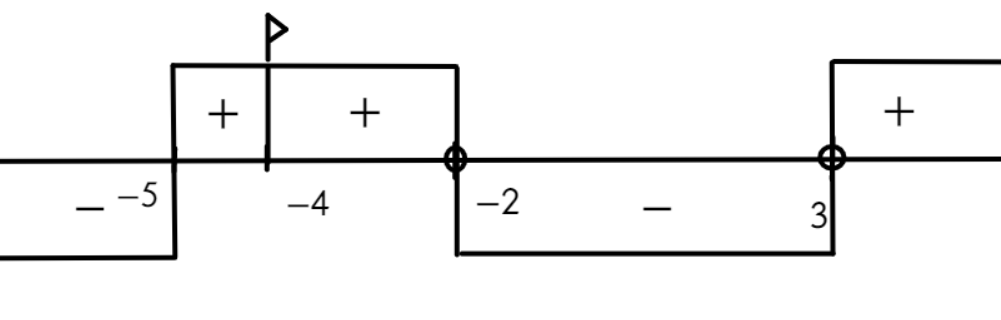
\includegraphics[scale=0.35]{isl3.png}}
\end{figure}
$x\in[-5;-2)\cup(3;+\infty).$\\
